\chapter{ဒေတာ၊ အိပ်စ်ပရက်ရှင်းနဲ့ ဗေရီရေဘဲလ်များ} \label{ch:ch05}
% Karel programming
%   basic syntax, problem solving skills with programming. conditionals, loops, recursion 
% data, data types
%   အခု တကယ့် ပရိုဂရမ်တွေ
% operations on data
% variables

ရှေ့ပိုင်း ကားရဲလ်အခန်း လေးခုမှာ လေ့လာခဲ့ကြတဲ့ အကြောင်းအရာတွေဟာ ပရိုဂရမ်မင်း ဘာသာရပ်ရဲ့ အခြေခံအကျဆုံး ပင်မထောက်တိုင် သဘောတရားတွေလို့ ဆိုရမှာပါ။ ဒီသဘောတရားတွေ မကျေညက်ဘဲ ပရိုဂရမ်ရေးလို့ မရပါဘူး။ ကွန်ဒီရှင်နယ်တွေဖြစ်တဲ့ \fCode{if}, \fCode{if...else}၊ ပြန်ကျော့ခြင်းအတွက် \fCode{for} နဲ့ \fCode{while} \fEn{loop}၊ ဖန်ရှင်တွေ၊ \fEn{top-down, bottom-up} ပရိုဂရမ်းမင်း၊ ရီကားရှင်းနဲ့ ရီကားဆစ်ဖ် စဉ်းစားခြင်း စတာတွေနဲ့ ပရိုဂရမ်းမင်း ပုစ္ဆာတွေ ဖြေရှင်းနိုင်ရင် ပရိုဂရမ်မာလှေကား ပထမ တစ်ထစ် တက်လှမ်းအောင်မြင်ပြီ ပြောနိုင်ပါတယ်။ ဒီသဘောတရားတွေကို ဘီဂင်နာတွေ အရိုးရှင်းဆုံးနည်းနဲ့ နားလည်အောင်၊ လေ့ကျင့်လို့ရအောင် ကားရဲလ်က ထောက်ကူပေးတာပါ။ စက်ရုပ်လေး ကားရဲလ်ကို နှုတ်ဆက်ခဲ့ပြီး အခု ဆက်လက်လေ့လာကြမှာကတော့ ဒေတာ၊ အိပ်စ်ပရက်ရှင်းနဲ့ ဗေရီရေဘဲလ်တွေ အကြောင်းပါ။ 

ကွန်ပျူတာတွေဟာ အချက်အလက်(ဒေတာ) အမျိုးမျိုးကို ကိုင်တွယ်ဆောင်ရွက်ပေးနိုင်တယ်။ ကိန်း\allowbreak ဂဏန်းတွေအပြင် စာသား၊ ရုပ်သံ စတာတွေကိုပါ လက်ခံ အလုပ်လုပ်ပေးနိုင်တယ်။ ဒီလိုလုပ်ဆောင်နိုင်စွမ်းဟာ ကွန်ပျူတာတွေကို နယ်ပယ်ပေါင်းစုံမှာ တွင်တွင်ကျယ်ကျယ် အသုံးချလာရခြင်းရဲ့ အဓိက အကြောင်းအရင်း ဆိုရင်လည်း မမှားဘူး။

ဒေတာ အမျိုးအစား အများအပြားရှိပေမဲ့ အခြေခံအကျဆုံးက ကိန်းဂဏန်းတွေပါ။ ကွန်ပျူတာတွေကို စတင်တီထွင်ဖို့ ကြိုးစားလာကြတဲ့ အဓိက အကြောင်းအရင်းကလည်း ဂဏန်းသင်္ချာ အတွက်အချက်တွေကို လုပ်ဆောင်ရာမှာ လူတွေကို အကူအညီ ပေးဖို့အတွက်ပဲလို့ ဆိုနိုင်ပါတယ်။ ဒါ့အပြင် စာသား၊ ရုပ်သံ စတဲ့ အခြားဒေတာ အမျိုးအစားတွေကို ကွန်ပျူတာထဲမှာ ဖော်ပြသိမ်းဆည်းထားဖို့အတွက် ကိန်းဂဏန်းတွေကိုပဲ အသုံးပြုထားတယ်ဆိုတာ နောက်ပိုင်းမှာ နားလည်သိမြင် လာပါလိမ့်မယ်။ ဒါကြောင့်လည်း ယနေ့ခေတ် ကွန်ပျူတာတွေကို ဒစ်ဂျစ်တယ် ကွန်ပျူတာတွေလို့ ခေါ်တာဖြစ်တယ်။ ကိန်းဂဏန်းကို အခြေခံပြီး အလုပ်လုပ်တဲ့ ကွန်ပျူတာတွေပေါ့။ 

\section{ကိန်းဂဏန်းများ}
အခုအခန်းအတွက် ပရိုဂရမ်ကုဒ် အပိုင်းအစ အတိုအထွာလေးတွေကို အလွယ်တကူ  လက်\allowbreak တွေ့ စမ်းသပ်ကြည့်လို့ရအောင် \fEn{Python Console} ကို အသုံးပြုပါမယ်။ \fEn{VS Code} မှာ \fEnSnd{View} မီနူးမှ \fEnSnd{Terminal} ကိုဖွင့် (\fEnSnd{Ctrl + `} ရှော့ကတ်ကီးနဲ့ ဖွင့်လို့လည်းရတယ်) ပြီး \fEnSnd{python} ကွန်းမန်းနဲ့ ကွန်ဆိုးလ်ကို \fEn{run} ပါ။ \fEn{PyCharm} မှာဆိုရင် \fEnSnd{Python Console} အိုင်ကွန်နှိပ်ပြီး \fEn{run} ပါ $\big\llbracket$ပုံ (\fRefNo{\ref{fig:vscconsole}})၊ (\fRefNo{\ref{fig:pycharmconsole}})$\big\rrbracket$။


\begin{figure}[tbh!]
\begin{tikzpicture}
  \node[anchor=south west,inner sep=0] (image) at (0,0)
  {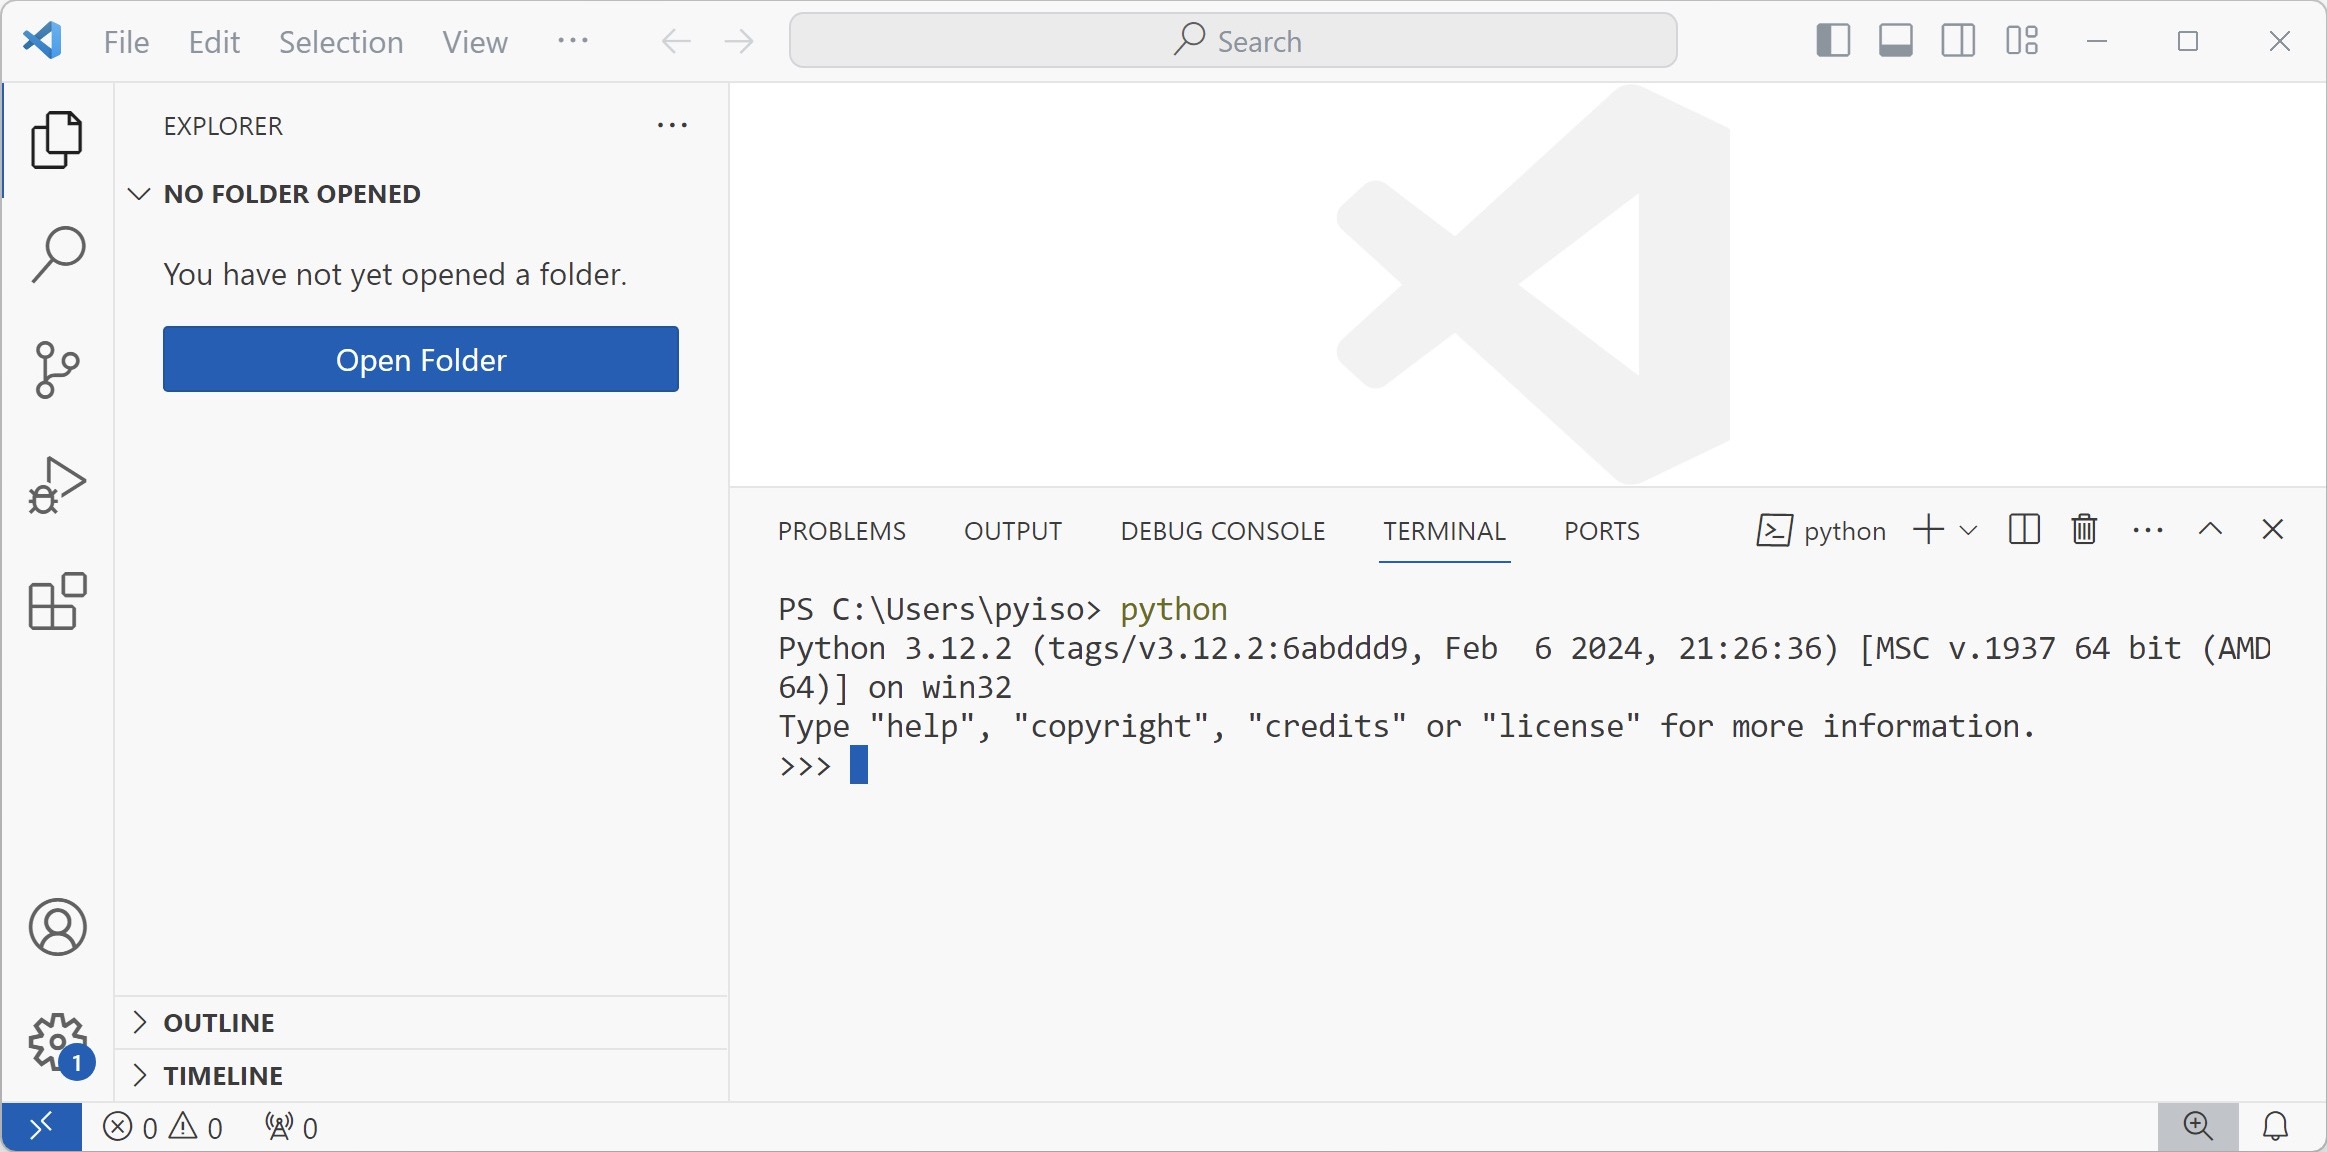
\includegraphics[width=.98\textwidth, trim={3mm 2mm 2mm 2.5mm},clip]{images/ch05/vscode py console.jpg}};
  \drawshadow{image}
\end{tikzpicture}
\caption{VS Code Python Console} 
\label{fig:vscconsole}
\end{figure}

\begin{figure}[tbh!]
\begin{tikzpicture}
  \node[anchor=south west,inner sep=0] (image) at (0,0)
  {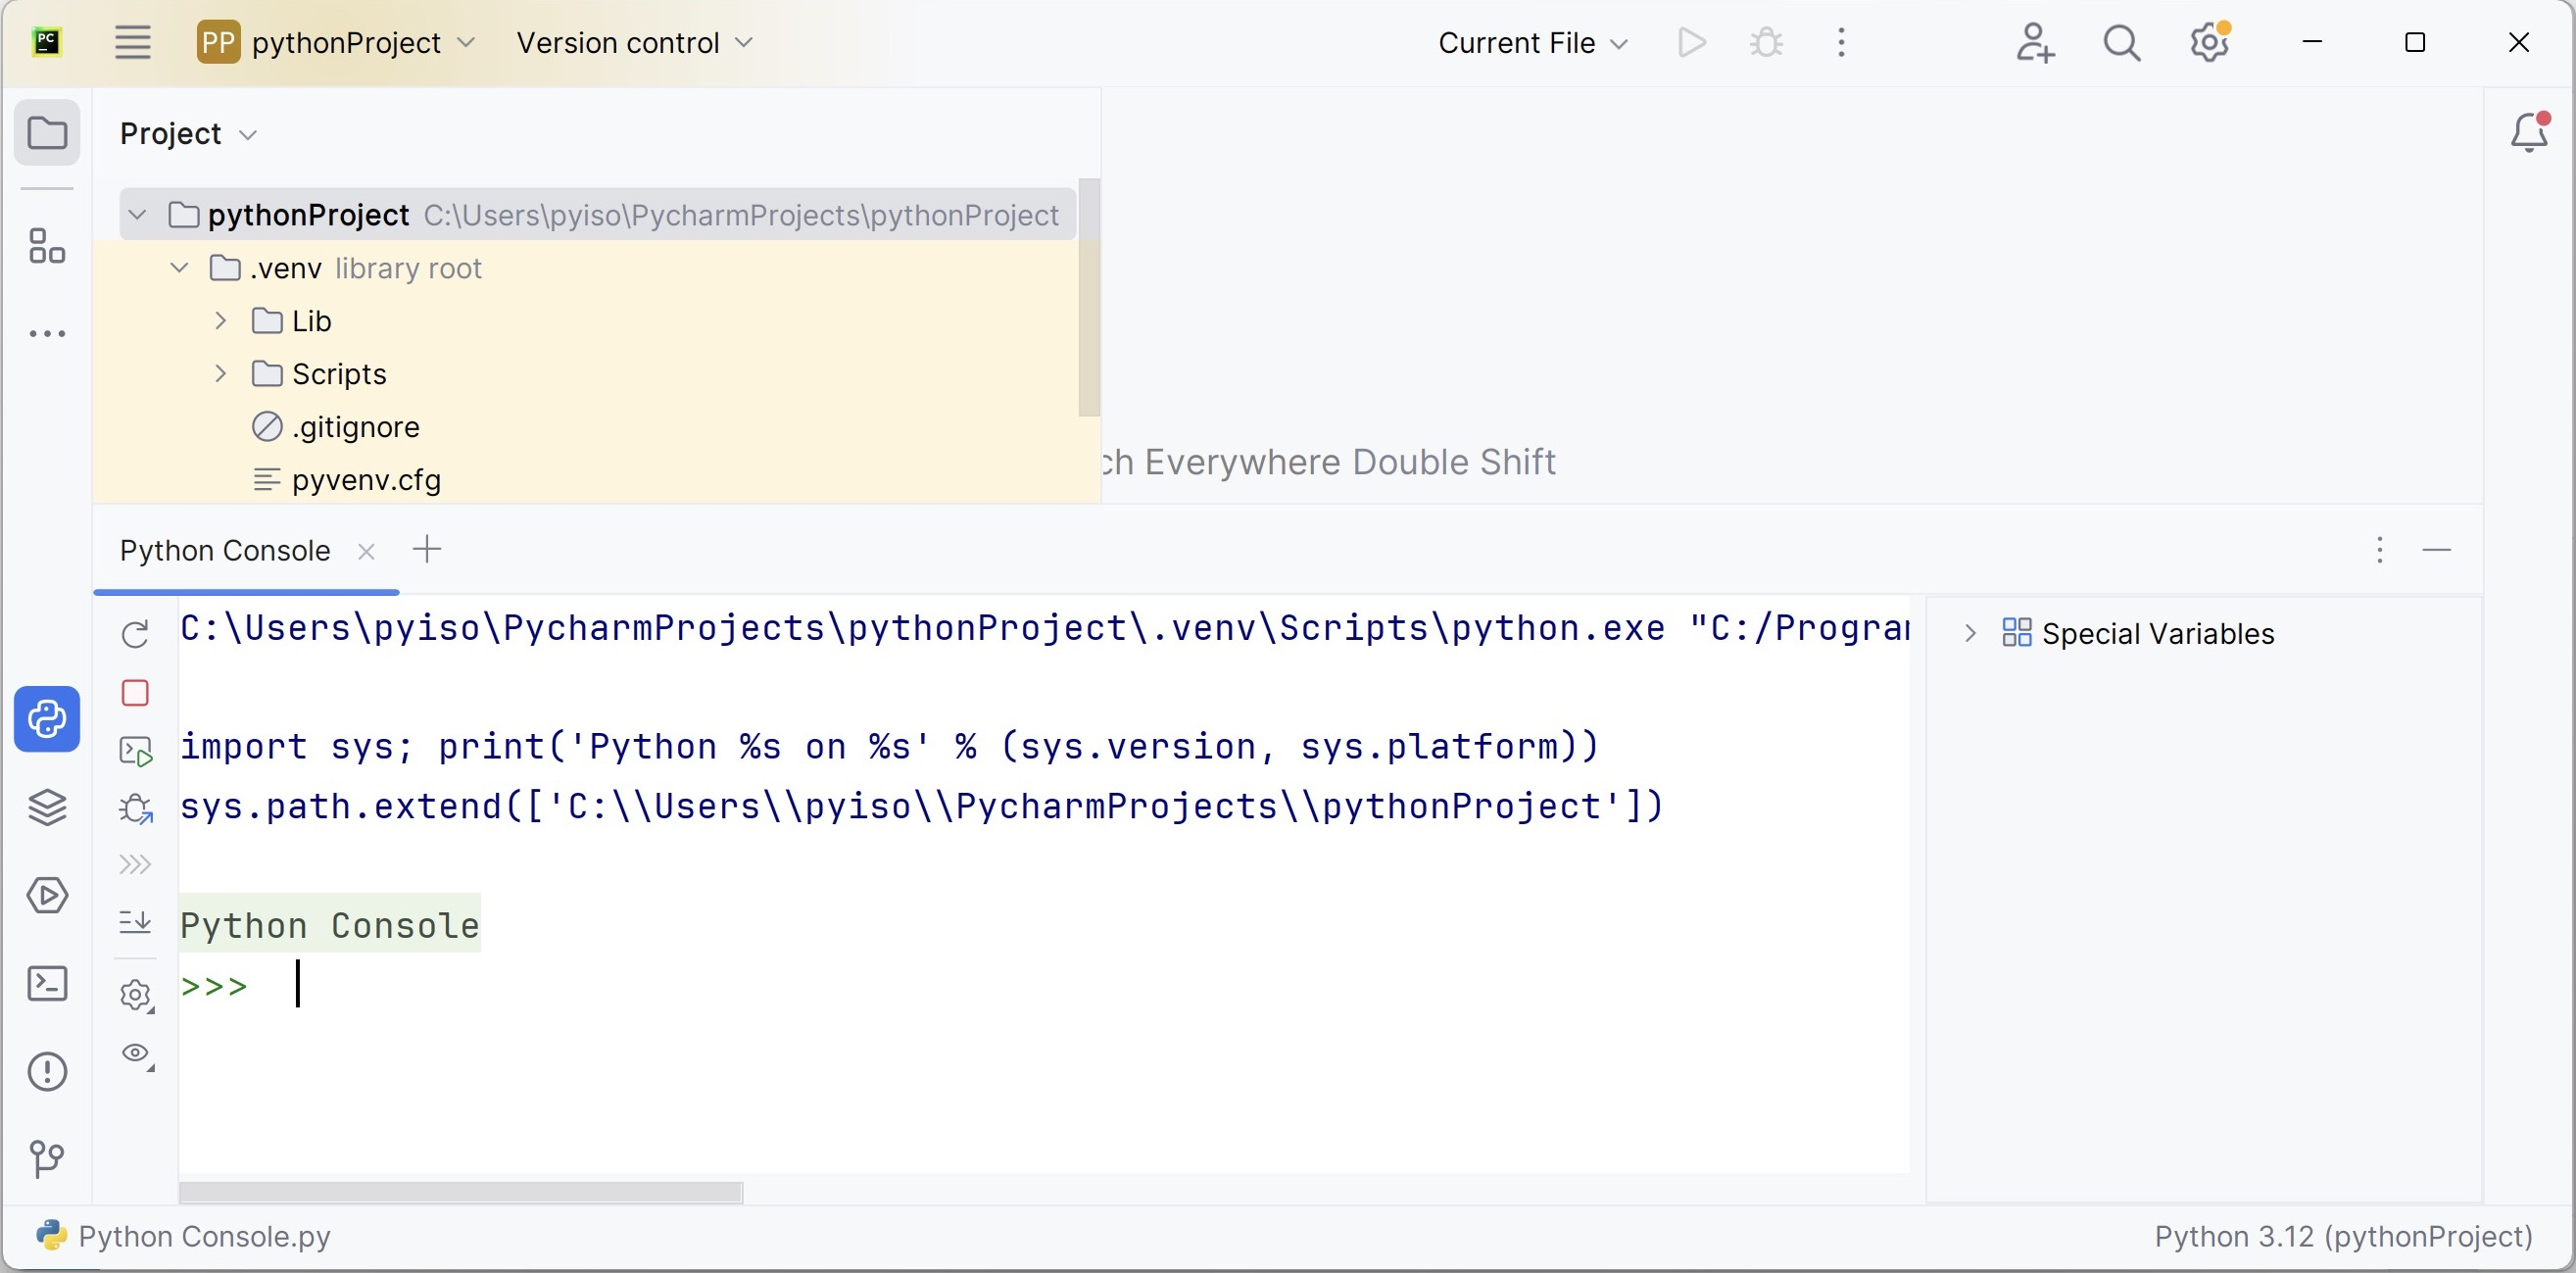
\includegraphics[width=.98\textwidth, trim={3mm 2mm 2mm 3.5mm},clip]{images/ch05/pycharm py console.jpg}};
  \drawshadow{image}
\end{tikzpicture}
\caption{PyCharm Python Console} 
\label{fig:pycharmconsole}
\end{figure}

ကွန်ဆိုးလ်မှာ \fCode{2 + 5} ထည့်ပြီး \fEn{Enter} ကီးနှိပ်ပါ။ အဖြေ \fCode{7} ထုတ်ပေးတာ တွေ့ရပါမယ်။
%
\setlength{\fboxsep}{0pt}
\begin{codetxt}
>>> 2 + 5;
7
\end{codetxt}
%
အောက်ပါအတိုင်း တစ်ခုပြီးတစ်ခု ဆက်လက်စမ်းသပ်ကြည့်ပါ။
%
\setlength{\fboxsep}{0pt}
\begin{codetxt}
>>> 2 + 2
4
>>> 3 * 3
9
>>> 4 - 2
2
>>> 5/2
2.5
\end{codetxt}
%
$3 \times 3$ ကို \fCode{3 * 3} လို့ ရိုက်ထည့်ပေးရပြီး $5 \div 2$ အတွက် \fCode{5 / 2} လို့ ရေးရတာကို သတိပြုမိမှာပါ။ \fEn{Programming language} အများစုမှာ \fCode{*} \fEn{(asterisk)} အမြှောက်သင်္ကေတအဖြစ် အသုံးပြုပြီး \fCode{/} \fEn{(forward slash)} ကို အစားသင်္ကေတအနေနဲ့ အသုံးပြုလေ့ရှိတယ်။

\subsection*{Values and Types}
တန်ဖိုးတိုင်းဟာ တိုက်ပ် \fEn{(\textit{type})} တစ်မျိုးမျိုးမှာ ပါဝင်ပါတယ်။  \fCode{-3}\fEn{,} \fCode{0}\fEn{,} \fCode{2}  စတဲ့ တန်ဖိုးတွေဟာ \fCode{int} (\fEn{integer} ရဲ့ အတိုကောက်) တိုက်ပ်ဖြစ်ပြီး 
\fCode{-3.0}\fEn{,} \fCode{0.1}\fEn{,} \fCode{3.3333} စတာတွေက \fCode{float} တိုက်ပ် ဖြစ်ပါတယ်။ ဒဿမကိန်းတွေကို ကွန်ပျူတာနဲ့ ဖော်ပြဖို့ \fEnEmp{floating point} လို့ခေါ်တဲ့ နည်းစနစ်ကို အသုံးပြုတယ်။ ဒဿမကိန်း အတွက်အချက်တွေကိုလည်း ဒီနည်းစနစ်ကို အခြေခံပြီး ကွန်ပျူတာက လုပ်ဆောင်တာပါ။ ဒါကြောင့် \fEn{floating point} ဟာ ဒဿမကိန်းတွေကို ဖော်ပြဖို့နဲ့ ဒဿမကိန်း အတွက်အချက်တွေ လုပ်ဆောင်ဖို့ တီထွင်ထားတဲ့ နည်းစနစ်တစ်ခုလို့ ဆိုနိုင်ပါတယ်။ ဒီစနစ်ကို အခြေခံထားတဲ့ ဒဿမကိန်းတွေကို \fEn{programming language} တွေမှာ \fCode{float} တိုက်ပ်လို့ ခေါ်တာပါ။


\fCode{float} တိုက်ပ်ဟာ လိုသလောက် တိကျလို့မရတဲ့ သဘောရှိတယ်။ အောက်ပါအတိုင်း စမ်းကြည့်ရင်  \fCode{0.3} နဲ့ \fCode{1.0} ရသင့်တာ ဖြစ်ပေမဲ့ အတိအကျ အဖြေမထွက်ပါဘူး။
%
\setlength{\fboxsep}{0pt}
\begin{codetxt}
>>> 0.1 + 0.1 + 0.1
0.30000000000000004
>>> 0.1 + 0.1 + 0.1 + 0.1 + 0.1 + 0.1 + 0.1 + 0.1 + 0.1 + 0.1;
0.9999999999999999
\end{codetxt}
%
ကွာခြားချက်က မဆိုစလောက် သေးငယ်တယ် ဆိုပေမဲ့ ဒီအချက်ကို ပရိုဂရမ်မာ အနေနဲ့ ဂရုပြုမိဖို့ လိုပါတယ်။  \fEn{Floating point}  စနစ်ဟာ လုံးဝကြီးတိကျဖို့ မလိုအပ်တဲ့ (တနည်းအားဖြင့် မဆိုစလောက်သေးငယ်တဲ့ ကွာဟချက်ကို လက်ခံနိုင်တဲ့) ကိန်းဂဏန်းအတွက်အချက် ကိစ္စတွေအတွက် ရည်ရွယ်တာပါ။ သိပ္ပံနဲ့ နည်းပညာဆိုင်ရာ တိုင်းတာ တွက်ချက်မှုတွေအတွက် အသုံးပြုလေ့ရှိတယ်။ ဒဿမကိန်းတွေ လုံးဝအတိအကျ ဖြစ်ဖို့ လိုအပ်တဲ့ ကိစ္စမျိုးတွေ (ဥပမာအားဖြင့် ငွေကြေးကိစ္စ အတွက်အချက်) မှာ အသုံးမပြုသင့်ပါဘူး။ ဆယ်ပြားကို \fCode{0.1} နဲ့ဖော်ပြရင် ဆယ်ပြားစေ့ ဆယ်စေ့ဟာ တစ်ကျပ် ဖြစ်ကို ဖြစ်သင့်ပြီး \fCode{0.9999999999999999} မဖြစ်သင့်ဘူး။ ဒီလိုကိစ္စမျိုးတွေအတွက် \fEn{Python} မှာ \fCode{Decimal} ကို အသုံးပြုနိုင်ပါတယ်။  လောလောဆယ် ကိန်းဂဏန်းတွေနဲ့ ပါတ်သက်ပြီး စကတည်းက သိထားသင့်တာတချို့ကို ကြိုပြောထားတာပါ။ \fCode{Decimal} တိုက်ပ် အကြောင်း မကြာခင် လေ့လာမှာပါ။
%
\setlength{\fboxsep}{0pt}
\begin{codetxt}
>>> from decimal import *
>>> Decimal('0.1') + Decimal('0.1') + Decimal('0.1')
Decimal('0.3')
\end{codetxt}
%

 \fCode{int}  တိုက်ပ် ဖော်ပြနိုင်တဲ့ အကြီးဆုံး အပေါင်းကိန်းပြည့် သို့မဟုတ် အငယ်ဆုံး အနှုတ်ကိန်းပြည့် တန်ဖိုးကို ကန့်သတ်ထားတာ မရှိဘူး။  သီအိုရီအရ ကြိုက်သလောက် ကြီးလို့/ငယ်လို့ ရပါတယ်။ လက်တွေ့မှာတော့ အသုံးပြုတဲ့ ကွန်ပျူတာစနစ်ပေါ် မူတည်ပြီး ကန့်သတ်ချက်ရှိမှာပါ။ ဒီစာရေးနေတဲ့ ကွန်ပျူတာမှာ အောက်ပါကိန်းပြည့်တွေကို အသာလေး တွက်ချက်ပေးနိုင်ပါတယ်။ ဒီ့ထက်အများကြီး ကြီးတဲ့ဟာတွေကိုလည်း ကိုင်တွယ်တွက်ချက်နိုင်အုံးမှာပါ။ တော်ရုံကိစ္စတွေအတွက် ကွန်ပျူတာစနစ်တစ်ခုရဲ့ လက်တွေ့ကန့်သတ်ချက်ကို ကျော်လွန်သွားဖို့ မလွယ်ပါဘူး။
%
\setlength{\fboxsep}{0pt}
\begin{codetxt}
>>> 9000000000000000000000000000 + 5000000000
9000000000000000005000000000
>>> -9000000000000000000000000000 + 1 
-8999999999999999999999999999
 \end{codetxt}
 %
 
 \fCode{float} ကတော့ \fCode{int} နဲ့ မတူဘဲ အကြီးဆုံး/အငယ်ဆုံး ကန့်သတ်ချက်ရှိပါတယ်။ ဒီကန့်သတ်ချက်ကလည်း ကွန်ပျူတာစနစ်ပေါ် မူတည်ပါတယ်။ တစ်ကိုယ်ရေသုံး ကွန်ပျူတာ အများစုအတွက် \(1 \times 10^{400}\) (၁ နောက် သုည အလုံး ၄၀၀) သို့မဟုတ် \(-1 \times 10^{400}\) (အနှုတ် ၁ နောက် သုည အလုံး ၄၀၀) ဟာ ကန့်သတ်ချက်ကျော်လွန်ပါတယ်။ 
%
\setlength{\fboxsep}{0pt}
\begin{codetxt}
>>> 1e400
inf
>>> -1e400
-inf
>>> 1e-400
0.0
>>> -1e-400
-0.0
 \end{codetxt}
 %
 ဒဿမကိန်းကို \fEnEmp{e} အမှတ်အသားနဲ့ရေးထားတာပါ။  အက္ခရာ \fCode{e} နောက် လိုက်တဲ့ ကိန်းပြည့်ဂဏန်းကို $10$ ထပ်ကိန်းလို့ မှတ်ယူရပါတယ်။ \fCode{e3} က \(1 \times 10^{3}\)\fEn{,} \fCode{e-3} က \(1 \times 10^{-3}\) ပါ။ အက္ခရာ \fEnEmp{E} အကြီးနဲ့လည်း ရေးနိုင်တယ်။ ထပ်ကိန်း ကြီးလွန်းတဲ့အတွက် ကန့်သတ်ချက် ကျော်လွန်ရင် \fCode{inf} (အနှုတ်ကိန်းဆိုရင် \fCode{-inf} ) ရပါမယ်။ \fEn{Infinity} ကို ဆိုလိုတာပါ။ (၁) မပြည့်တဲ့ ပမာဏ သေးငယ်လွန်းတဲ့ ဂဏန်းတွေကိုလည်း အနီးစပ်ဆုံး သုညအနေနဲ့ ယူပါတယ်။ အနီးစပ်ဆုံးယူတဲ့အခါ အပေါင်း/အနှုတ်ကိုတော့ ခွဲခြားပေးပါတယ်။ \fEnEmp{e} အမှတ်အသားနဲ့ရေးထားတဲ့ နောက်ထပ် ဥပမာလေး နှစ်ခုပါ
%
\setlength{\fboxsep}{0pt}
\begin{codetxt}
7.34767309e22    # mass of the moon in kg
9.1093837015e-31 # mass of an electron in kg
\end{codetxt}
%

ဂဏန်းအလုံးအရေအတွက် များရင် $100,500$ (တစ်သိန်းငါးရာ)၊ $1,500,000$ (တစ်သန်းငါးသိန်း) စသဖြင့် သုံးလုံးတစ်ဖြတ် ကော်မာခံရေးလေ့ရှိတယ်။ \fEn{Python} မှာတော့ ကော်မာအစား \fEn{\textunderscore (underscore)} နဲ့ သုံးလုံးတစ်ဖြတ် ခြားရေးနိုင်ပါတယ်။ 
%
\setlength{\fboxsep}{0pt}
\begin{codetxt}
>>> 1_500_000 + 100_500
1600500
>>> 200_000.33 + 3_800_000.22
4000000.5500000003
\end{codetxt}
%



\subsection*{တိုက်ပ်မတူသည့် ကိန်းဂဏန်း အိပ်စ်ပရက်ရှင်များ}
အိပ်စ်ပရက်ရှင်တွေမှာ ပါဝင်တဲ့ တိုက်ပ် တစ်မျိုးတည်း ဖြစ်ရမယ် မရှိပါ။ တိုက်ပ်မတူတဲ့ ကိန်းဂဏန်းတွေ အိပ်စ်ပရက်ရှင်တစ်ခုမှာ ရောပြီး ပါဝင်နိုင်ပါတယ်။
%
\setlength{\fboxsep}{0pt}
\begin{codetxt}
>>> 5 - 2.0
3.0
>>> 5 - 2
3
>>> 3 * 2.0
6.0
>>> 3 * 2
6
\end{codetxt}
%
\fCode{int} နဲ့ \fCode{float} ရောနေရင် အိပ်စ်ပရက်ရှင် ရလဒ်သည် \fCode{float} တိုက်ပ် ဖြစ်မှာပါ။ အစား \fEn{(division)} မှာတော့ အင်တီဂျာအချင်းချင်း စားတဲ့အခါမှာလည်း ရလဒ်က \fCode{float} ဖြစ်ပါမယ်။ 
%
\setlength{\fboxsep}{0pt}
\begin{codetxt}
>>> 9/3
3.0
>>> 9.12/3.3
2.7636363636363637
>>> 88/3
29.333333333333332
>>> 1/3
0.3333333333333333
>>>
\end{codetxt}
%

\subsection*{အင်တီဂျာ ဒီဗီးရှင်း၊ မော်ဒျူလို နှင့် ထပ်ကိန်းတင်ခြင်း}
အကယ်၍ ဒဿမကိန်းမထွက်ဘဲ ကိန်းပြည့် လိုချင်ရင် \fCode{//} ကို သုံးရပါမယ်။ ဒီအခါ အကြွင်းကိုဖယ်ပြီး စားလဒ်ကိုပဲ ကိန်းပြည့်အနေနဲ့ ရမှာပါ။ 
%
\setlength{\fboxsep}{0pt}
\begin{codetxt}
>>> 9//3
3
>>> 12//5
2
>>> 3//5
0
\end{codetxt}
%
သင်္ချာမှာ ဒီလိုမျိုး အစားကို အင်တီဂျာ ဒီဗီးရှင်း \fEn{(integer division)} လို့ခေါ်ပါတယ်။ အကြွင်းရှာမယ်ဆိုရင် \mintinline{text}|%| အော်ပရိတ်တာ ရှိပါတယ်။ \mintinline{text}|%| ကို မော်ဒျူလို \fEn{(modulo)} အော်ပရိတ်တာလို့ ခေါ်တယ်။ \fEn{remainder} အော်ပရိတ်တာလို့လည်း ခေါ်တယ်။ 
%
\setlength{\fboxsep}{0pt}
\begin{codetxt}
>>> 7 % 5
2
>>> 100 % 10
0
\end{codetxt}
%

အင်တီဂျာ ဒီဗီးရှင်းနဲ့ မော်ဒျူလိုကို အနှုတ်ကိန်းတွေနဲ့ သုံးမယ်ဆိုရင် သတိပြုပါ။  စားလဒ် အနှုတ်ကိန်း ဖြစ်ရင် \fCode{//} က ပိုငယ်တဲ့ အနှုတ်ကိန်းကို အနီးစပ်ဆုံး ယူမှာပါ။ တစ်နည်းအားဖြင့် \fEn{round down} လုပ်တာ ဖြစ်တယ်။
%
\setlength{\fboxsep}{0pt}
\begin{codetxt}
>>> -12 // -10
1
>>> -12 // 10
-2
>>> 12 // -10
-2
>>> -31 // 10
-4
>>> -35 // 10
-4
>>> -38 // 10
-4
\end{codetxt}
%
\fCode{-2} နဲ့ \fCode{-4} ထွက်တာ သတိပြုပါ။ အဖြေအတိအကျက \fCode{-1.2} ကို အနီးစပ်ဆုံး သူ့ထက်ပိုငယ်တဲ့ \fCode{-2} ကို အနီးစပ်ဆုံး ယူတယ်။ \fCode{-3.1}\fEn{,} \fCode{-3.5}\fEn{,} \fCode{-3.8} တို့ကိုလည်း အနီးစပ်ဆုံး \fCode{-4} ယူတာပါ။

မော်ဒျူလို အော်ပရိတ်တာ \mintinline{text}|%| သုံးတဲ့အခါ ရလဒ်ဟာ စားကိန်းရဲ့ \fEn{sign} အပေါ် မူတည်တယ်။ (အပေါင်း အနှုတ်ကို ဆိုလိုတာပါ)။ 
%
\setlength{\fboxsep}{0pt}
\begin{codetxt}
>>> -17 % 10
3
>>> 17 % -10
-3
\end{codetxt}
%
မော်ဒျူလိုနဲ့ အင်တီဂျာ ဒီဗီးရှင်း အော်ပရိတ်တာ နှစ်ခုက အောက်ပါညီမျှခြင်းအရ ဆက်စပ်နေတာပါ။ စားကိန်း $B \neq 0$ ဖြစ်ပါတယ်။
\[
  B * (A // B) + A \SI{}{\fEn{\percent}} B = A
\]
ဒါကြောင့် $B = 10, A = -17$ ဖြစ်လျှင် 
\begin{align*}
B * (A//B) + A \SI{}{\fEn{\percent}} B &= A &\\
10 * (-17//10) + -17 \SI{}{\fEn{\percent}} 10 &= -17 &\\
-20 + -17 \SI{}{\fEn{\percent}} 10 &= -17 &\\
-17 \SI{}{\fEn{\percent}} 10 &= -17 + 20 &\\
-17 \SI{}{\fEn{\percent}} 10 &= 3 &
\end{align*}
အကယ်၍ $B = -10, A = 17$ ဖြစ်လျှင်
\begin{align*}
B * (A//B) + A \SI{}{\fEn{\percent}} B &= A&\\
-10 * (17//-10) + 17 \SI{}{\fEn{\percent}} -10 &= 17&\\
20 + 17 \SI{}{\fEn{\percent}} -10 &= 17&\\
17 \SI{}{\fEn{\percent}} -10 &= 17 - 20&\\
17 \SI{}{\fEn{\percent}} -10 &= -3 &
\end{align*}

အထက်ပါ ညီမျှခြင်းဟာ ကိန်းပြည့်တွေအတွက်ပဲ မှန်တာပါ။ \fCode{//} နဲ့ \mintinline{text}|%|  ကို ဒဿမကိန်းတွေနဲ့လည်း သုံးလို့ရပေမဲ့ ရလဒ်တွေက အထက်ပါ ညီမျှခြင်းကို ပြေလည်စေမှာ မဟုတ်ပါဘူး။ \fCode{float} တိုက်ပ်ဟာ 
%
\setlength{\fboxsep}{0pt}
\begin{codetxt}
>>> 9.9 // 3.3
3.0
>>> 9.9 % 3.3
8.881784197001252e-16
>>> 9.9 / 3.3
3.0000000000000004
>>> 3.5 / 0.1
35.0
>>> 3.5 // 0.1
34.0
>>> 3.5 % 0.1
0.09999999999999981
\end{codetxt}
%


ထပ်ကိန်းတင် \fEn{(exponentiation)} ဖို့ အတွက် အော်ပရိတ်တာက \fCode{**}  ပါ။ $2^4$ နဲ့ $(3.3)^3$ ကို အခုလို တွက်ပါတယ်။
%
\setlength{\fboxsep}{0pt}
\begin{codetxt}
>>> 2 ** 4
16
>>> 3.3 ** 3
35.937
\end{codetxt}
%

\subsection*{သင်္ချာဖန်ရှင်များ}
ကိန်းဂဏန်းတွေအကြောင်း လေ့လာလက်စနဲ့ \fCode{math} လိုက်ဘရီ သင်္ချာဖန်ရှင်တချို့ကိုလည်း တစ်ခါတည်း ဆက်ကြည့်လိုက်ရအောင်။ အဓိကက သင်္ချာဖန်ရှင်ဆိုတာထက် ဖန်ရှင် အခြေခံအသုံးပြုပုံကို စပြီးလေ့လာမှာပါ။ \fCode{math} လိုက်ဘရီက \fEn{Python} မှာ တစ်ခါတည်း ထည့်ထားပေးပြီးသား \fEn{(built-in)} လိုက်ဘရီပါ။ အင်စတောလ်လုပ်စရာ မလိုဘဲ အင်ပို့လုပ်ပြီး သုံးလို့ရတယ်။
\begin{codetxt}
>>> from math import *
\end{codetxt}
အင်ပို့လုပ်ပြီးရင် \fCode{math} လိုက်ဘရီဖန်ရှင်တွေကို သုံးလို့ရပါပြီ။ ကိန်းတစ်ခုရဲ့ နှစ်ထပ်ကိန်းရင်းကို \fCode{sqrt}\fEn{,} သုံးထပ်ကိန်းရင်းကို \fCode{cbrt} ဖန်ရှင်နဲ့ ရှာနိုင်ပါတယ်။
\begin{codetxt}
>>> cbrt(27)
3.0
>>> sqrt(81)
9.0  
\end{codetxt}

သင်္ချာဖန်ရှင်အားလုံးဟာ \fEn{input} တန်ဖိုးတစ်ခု သို့မဟုတ် တစ်ခုထက်ပို၍ လက်ခံပြီး \fEn{output} တန်ဖိုးတစ်ခု ပြန်ထုတ်ပေးပါတယ်။ \fCode{27} နဲ့  \fCode{81} ဟာ \fEn{input} ဖြစ်ပြီး \fCode{3.0} နဲ့  \fCode{9.0} က \fEn{output} ဖြစ်တယ်။
\begin{codetxt}
>>> gcd(2406, 654)
6
>>> gcd(2406, 654, 354)
6
>>> gcd(2406)
2406
\end{codetxt}
အကြီးဆုံးဘုံဆခွဲကိန်းကို \fCode{gcd} ဖန်ရှင်နဲ့ ရှာတာပါ။ အင်တီဂျာ \fEn{input} တစ်ခုနဲ့အထက် လက်ခံတဲ့ ဖန်ရှင်ဖြစ်တယ်။ \fEn{input} ဂဏန်းအားလုံးကို စားလို့ပြတ်တဲ့ အကြီးဆုံးကိန်းကို ရှာပေးတယ်။ ကိန်းပြည့်မဟုတ်တာ ထည့်ရင် အယ်ရာဖြစ်ပါတယ်။
\begin{codetxt}
>>> gcd(2.4, 4.8)
Traceback (most recent call last):
  File "<stdin>", line 1, in <module>
TypeError: 'float' object cannot be interpreted as an integer
\end{codetxt}

လော့ဂရစ်သမ်၊ ထရီဂိုနိုမေထရီ ဖန်ရှင်တွေလည်းပါတယ်။ $\log_{10}(x)$\fEn{,} $\sin(x)$\fEn{,} $\cos(x)$ တို့ကို ဥပမာပြထားတာ ကြည့်ပါ။
\begin{codetxt}
>>> log10(1000)
3.0
>>> sin(pi/2) # pi/2 radians = 90 degrees
1.0
>>> sin(pi/4) ** 2 + cos(pi/4) ** 2
1.0
\end{codetxt}


\section{‘တိုက်ပ်’ ဆိုတာ ဘာလဲ}
\fEn{Programming language} အားလုံးမှာ တိုက်ပ် သဘောတရား ပါရှိပါတယ်။ \fCode{int} နဲ့ \fCode{float} တိုက်ပ်မှာ ပါဝင်တဲ့ ကိန်းပြည့်တွေနဲ့ ဒဿမကိန်းတွေကို မိတ်ဆက်ပြီးတဲ့အခါ ‘တိုက်ပ်’ ဆိုတာဘာလဲ တိတိကျကျ ရှင်းပြလို့ရပါပြီ။ တိုက်ပ်တစ်ခုဟာ
%
\begin{itemize}
  \item တန်ဖိုးတွေပါဝင်တဲ့ အစု \fEn{(set)} တစ်ခု နဲ့
  \item ၎င်းတန်ဖိုးများအပေါ်တွင် အသုံးချနိုင်တဲ့ အော်ပရေးရှင်းတွေ ပါဝင်တဲ့ အစုတစ်ခု
\end{itemize}
%
ဖြစ်ပါတယ်။ ဥပမာ \fCode{int} တိုက်ပ်ကို ကြည့်ရင် ကိန်းပြည့်တွေ ပါဝင်တဲ့ အစုနဲ့ ကိန်းပြည့်တွေအပေါ်မှာ လုပ်ဆောင်လို့ရတဲ့  အော်ပရေးရှင်းတွေ ပါဝင်တဲ့ အစု
%
\begin{align*}
& \{\ldots , -3, -2, -1, 0, 1, 2, 3, \ldots \} &\\
& \{+, -, *, /, //, \SI{}{\fEn{\percent}}, **, \ldots \} &%
\end{align*}
ဖြစ်ပါတယ်။ \fCode{float} တိုက်ပ်ကတော့ ကိန်းစစ် \fEn{(real numbers)} တွေပါဝင်တဲ့ အစုနဲ့ ၎င်းတို့အပေါ်မှာ လုပ်ဆောင်လို့ရတဲ့  အော်ပရေးရှင်းတွေ ပါဝင်တဲ့ အစုတို့ ဖြစ်ပါတယ်။ \fCode{int} နဲ့ \fCode{float} တိုက်ပ်မှာ အော်ပရေးရှင်းတွေ တူတူဖြစ်နေတာ တွေ့ရမှာပါ။ ဒီလိုအမြဲဖြစ်မယ်လို့ မယူဆရပါဘူး။ တိုက်ပ် မတူတဲ့အခါ အသုံးချလို့ ရနိုင်တဲ့ အော်ပရေးရှင်းတွေ ကွာခြားနိုင်ပါတယ်။ ဥပမာ \fCode{str} တိုက်ပ် အော်ပရေးရှင်းတွေက \fCode{int} တို့ \fCode{float} တို့နဲ့ မတူပါဘူး။ \fCode{str} က \fEnEmp{string} ရဲ့ အတိုကောက်ဖြစ်ပြီး စာသားတွေအတွက် အသုံးပြုပါတယ်။ မကြာခင် လေ့လာကြမှာပါ။

အပေါ်က အော်ပရေးရှင်း အစုမှာ အစက်သုံးစက် $‘\ldots’$ ကို သတိပြုပါ။ ဆိုလိုတာက အခြား အော်ပရေးရှင်းတွေ ဒီအစုမှာ ပါဝင်ပါသေးတယ်။ \fCode{int} နဲ့ \fCode{float} တွေအတွက် ဖန်ရှင်တွေကိုလည်း ဒီအစုမှာ ပါဝင်တယ်လို့ ယူဆရမှာပါ။
%
\setlength{\fboxsep}{0pt}
\begin{codetxt}
>>> from math import *
>>> sqrt(2.0)
1.4142135623730951
>>> abs(-5)
5
\end{codetxt}
% 
ဥပမာအနေနဲ့ \fCode{sqrt} နဲ့ \fCode{abs} ဖန်ရှင် အသုံးချပုံပါ။ နှစ်ထပ်ကိန်းရင်းနဲ့ ပကတိတန်ဖိုး ရှာပေးပါတယ်။ လိုအပ်ရင် ကိုယ်ပိုင်ဖန်ရှင်တွေ သတ်မှတ်ပြီး တိုက်ပ်တစ်ခုရဲ့ အော်ပရေးရှင်းတွေကို ဖြည့်စွက်တိုးချဲ့နိုင်ပါတယ်။

\begin{mytcbox}
အော်ပရေးရှင်းနဲ့ အော်ပရိတ်တာ ရောထွေးစရာ ရှိပါတယ်။ $+, -, *, /, //, \SI{}{\fEn{\percent}}, **$ စတဲ့ သင်္ကေတတွေကို အော်ပရိတ်တာလို့ ခေါ်ပါတယ်။ အော်ပရေးရှင်း လုပ်ဆောင်ဖို့အတွက် အသုံးပြုတဲ့ သင်္ကေတတွေကို အော်ပရိတ်တာလို့ ခေါ်တာပါ။ ဥပမာ “$*$ သင်္ကေတဟာ အမြှောက်အော်ပရေးရှင်း လုပ်ဆောင်ဖို့ သတ်မှတ်ထားတဲ့ အော်ပရိတ်တာ” လို့ ပြောတယ်။ အမြှောက်  ‘အော်ပရေးရှင်း’ ကျတော့ မြှောက်တဲ့အလုပ် ဆောက်ရွက်တာကို ဆိုလိုတာ။
\end{mytcbox}


\section{ဗေရီရေဘဲလ်များ}
ဗေရီရေဘဲလ်ဆိုတာ တန်ဖိုးတစ်ခုကို ကိုယ်စားပြုတဲ့ နံမည်ပါပဲ။ နံမည်နဲ့ ၎င်းကိုယ်စားပြုတဲ့ တန်ဖိုး တွဲဖက်ပေးဖို့ အဆိုင်းမန့် \fEn{(\textit{assignment})} စတိတ်မန့်ကို သုံးရပါတယ်။
%
\setlength{\fboxsep}{0pt}
\begin{codetxt}
>>> age = 12
>>> weight = 35.5
\end{codetxt}
%
\fCode{age} နဲ့ \fCode{weight} ဟာ ဗေရီရေဘဲလ်တွေ ဖြစ်ပါတယ်။   ညီမျှခြင်းသင်္ကေတ (\fCode{=}) ကတော့ အဆိုင်းမန့် အော်ပရိတ်တာပါ။ ဗေရီရေဘဲလ်နဲ့ တန်ဖိုး တွဲဖက်ပေးတဲ့ အော်ပရိတ်တာ ဖြစ်တယ်။ ဗေရီရေဘဲလ်နံမည်ကို \fEn{variable} \fEnEmp{identifier} လို့လည်း ခေါ်ပါတယ်။ \fEn{Identifier} က နည်းပညာ အခေါ်အဝေါ်ပေါ့။ \fEn{Variable name} က သာမန်လူ နားလည်တဲ့ နည်းနဲ့ ပြောတာပါ။ ဗေရီရေဘဲလ် တစ်ခုချင်း ထည့်ကြည့်ရင် ၎င်းကိုယ်စားပြုတဲ့ တန်ဖိုးကို ပြန်ထုတ်ပေးတာ တွေ့ရမှာပါ။
%
\setlength{\fboxsep}{0pt}
\begin{codetxt}
>>> age
12
>>> weight
35.5
\end{codetxt}

%
အိပ်စ်ပရက်ရှင်တွေက ဗေရီရေဘဲလ်တွေနဲ့ ဖြစ်နိုင်ပါတယ်။ အိပ်စ်ပရက်ရှင် တွက်ချက်ရင် ‌ဗေရီရေဘဲလ် တန်ဖိုးနဲ့ အစားထိုး တွက်ချက်တယ်လို့ ယူဆရမှာပါ။ ဥပမာ
%
\setlength{\fboxsep}{0pt}
\begin{codetxt}
>>> age + 1
13
>>> weight / 2
17.75
\end{codetxt}
%
ဗေရီရေဘဲလ်တစ်ခုကို အိပ်စ်ပရက်ရှင်ရလဒ်နဲ့ အဆိုင်းမန့် လုပ်လို့ရပါတယ်။ \fCode{rect\_area} ကို အောက်တွင် ကြည့်ပါ။ အလျား အနံ မြှောက်လဒ်ကို အဆိုင်းမန့် လုပ်ထားတာ တွေ့ရပါမယ်။
%
\setlength{\fboxsep}{0pt}
\begin{codetxt}
>>> rect_width = 22.5
>>> rect_length = 10
>>> rect_area = rect_width * rect_length
>>> rect_area
225.0
\end{codetxt}
%


\subsection*{အဆိုင်းမန့် စတိတ်မန့်}
ဗေရီရေဘဲလ်တစ်ခုဟာ အချိန်တစ်ချိန်မှာ တန်ဖိုးတစ်ခုကိုပဲ ကိုယ်စားပြုနိုင်တယ်။ ဒါပေမဲ့ အချိန်ကာလပေါ် မူတည်ပြီး တန်ဖိုးပြောင်းနိုင်တယ်။ (တစ်ချိန်တည်းမှာ တန်ဖိုးနှစ်ခု မဖြစ်နိုင်ဘူး)။ ဥပမာ \fCode{x} တန်ဖိုးဟာ ပထမ \fCode{10} ပါ။ ဒုတိယ အဆိုင်းမန့်လုပ်ပြီးတဲ့ အချိန်မှာ အဲ့ဒီ \fCode{x} ကပဲ \fCode{1000} ဖြစ်နေမှာပါ။ 
%အဆိုင်းမန့် စတိတ်မန့်မှာ \fEn{identifier} က အသစ်ဖြစ်နိုင်သလို ရှိပြီးသားလည်း ဖြစ်နိုင်ပါတယ်။ 
%
\setlength{\fboxsep}{0pt}
\begin{codetxt}
>>> x = 10
>>> x
10
>>> x = 1000
>>> x
1000
\end{codetxt}
%

\section{စာသားများ}
စာသား \fEn{(text)} ဟာ အသုံးအများဆုံး ဆက်သွယ်ဆောင်ရွက်ရေး ကြားခံနယ်တစ်ခုပါ။ ဝက်ဘ်ဆိုက် စာမျက်နှာ၊ အီးမေးလ်၊ အီးဘွတ်ခ်နဲ့ အီလက်ထရွန်းနစ် စာရွက်စာတမ်း \fEn{(e-documents)} စတာတွေမှာ ရုပ်သံတွေ အသုံးပြုလာကြပေမဲ့ စာသား အဓိကဖြစ်နေဆဲပါပဲ။ ဆိုရှယ်မီဒီယာ၊ ဂိမ်းနဲ့ အခြားအပ်ပ်တွေ ဟာလည်း စာသားနဲ့ မကင်းနိုင်ကြပါဘူး။ ဒါကြောင့် ပရိုဂရမ်းမင်းအတွက် စာသားဟာ  ဘယ်လောက်ထိ အရေးပါကြောင်း အများကြီးပြောစရာ လိုမယ်မထင်ပါဘူး။ 

ပရိုဂရမ်းမင်းမှာ စာသားကို \fEnEmp{string} လို့ခေါ်ပြီး ကာရက်တာ \fEn{(\textit{character})} တွေနဲ့ စီတန်းဖွဲ့စည်းထားတယ်။ ကာရက်တာဆိုတာ အခြေခံ သတင်းအချက်အလက် ယူနစ်တစ်ခုပါပဲ။ အက္ခရာ၊ ဂဏန်း \fEn{(digit)}၊ သင်္ကေတ သို့မဟုတ် ကွန်ထရိုးလ်ကုဒ် တစ်ခုခု ဖြစ်နိုင်ပါတယ်။ ဥပမာ \fEn{A, B, C, \$, @, \#, 1, 3, \_ } စသည်ဖြင့်။ \fEn{Double quotes(}\fCode{"}\fEn{)} တစ်စုံကြား ညှပ်ရေးထားတဲ့ ကာရက်တာတွေ အသီအတန်းလိုက်ကို စာသားအနေနဲ့ ယူဆတယ်။ \fEn{Python} မှာ စာသားရဲ့ တိုက်ပ်ဟာ \fCode{str} ဖြစ်တယ်။ \fEn{string} ကို အတိုကောက် ယူထားတာပါ။ 
%
\setlength{\fboxsep}{0pt}
\begin{codetxt}
>>> "Hello, World!"
'Hello, World!'
\end{codetxt}
%
သို့မဟုတ် \fCode{"} အစား \fEn{single quotes(}\fCode{'}\fEn{)} တစ်စုံလည်း သုံးနိုင်ပါတယ်။ 
%
\setlength{\fboxsep}{0pt}
\begin{codetxt}
>>> 'Hello, World!'
'Hello, World!'
\end{codetxt}
%

စာသားတစ်ခုမှာ ပါဝင်တဲ့ ကာရက်တာ အရေအတွက်ကို \fCode{len} ဖန်ရှင်နဲ့ စစ်ကြည့်နိုင်ပါတယ်။ ကာရက်တာ တစ်လုံးမှ မပါတဲ့ \fCode{""} (သို့ \fCode{''}) ကို \fEn{empty string} လို့ ခေါ်ပါတယ်။ 
%
\setlength{\fboxsep}{0pt}
\begin{codetxt}
>>> len("Hello, World!")
13
>>> long_sentence = "This is a long sentence nobody wants to read."
>>> len(long_sentence)
45
>>> len("")
0
>>> len(" ") # contain a single space
1
\end{codetxt}
%

\fCode{str} တိုက်ပ်ရဲ့ အခြေခံကျတဲ့ အော်ပရေးရှင်းတစ်ခုက စာသားတစ်ခုနဲ့ တစ်ခု ဆက်တာပါ။ \fCode{+} အော်ပရိတ်တာနဲ့ စာသားတွေကို ဆက်နိုင်ပါတယ်။ 
%အော်ပရိတ်တာတစ်ခုဟာ တွဲဖက်အသုံးပြုတဲ့ \fEn{operand} တွေရဲ့ တိုက်ပ်ပေါ်မူတည်ပြီး လုပ်ဆောင်တဲ့ အော်ပရေးရှင်း  \todo{ကိန်းဂဏန်းစက်ရှင်တွင် ကြိုရှင်းရန်}
%
\setlength{\fboxsep}{0pt}
\begin{codetxt}
>>> "Yangon " + "and " + "Mandalay"
'Yangon and Mandalay'
\end{codetxt}
%
စာသားအချင်းချင်းပဲ ဆက်လို့ရပါတယ်။ စာသားနဲ့ ကိန်းဂဏန်း ဆက်လို့မရပါဘူး။ အောက်ပါအတိုင်း စမ်းကြည့်တဲ့အခါ \fCode{str} နဲ့ \fCode{float} ဆက်လို့မရဘူးလို့ အယ်ရာ\fOpn{မက်ဆေ့ချ်} ကျလာမှာပါ။
%
\setlength{\fboxsep}{0pt}
\begin{codetxt}
>>> from math import *
>>> pi
3.141592653589793
>>> "The value of π is " + pi
Traceback (most recent call last):
  File "<stdin>", line 1, in <module>
TypeError: can only concatenate str (not "float") to str
\end{codetxt}
%
\fCode{str} ဖန်ရှင်က ကိန်းဂဏန်းတစ်ခုကနေ စာသားကို ထုတ်ပေးပါတယ်။ မူရင်းကိန်းဂဏန်းကို စာသားဖြစ်အောင် ပြောင်းလိုက်တာ မဟုတ်ပါဘူး။ ကိန်းဂဏန်း တန်ဖိုးကနေ ၎င်းကိုဖော်ပြတဲ့ စာသားကို ဖန်ရှင်က ပြန်ထုတ်ပေးတာပါ။ 
%
\setlength{\fboxsep}{0pt}
\begin{codetxt}
>>> str(pi)
'3.141592653589793'
\end{codetxt}
%
ထွက်လာတဲ့ တန်ဖိုးဟာ စာသားဖြစ်တဲ့အတွက် \fEn{single quote} ပါနေတာ သတိပြုပါ။ \fCode{pi} တန်ဖိုးနဲ့ စာသား အခုလို ဆက်ရပါမယ်။ 
%
\setlength{\fboxsep}{0pt}
\begin{codetxt}
>>> "The value of π is " + str(pi)
'The value of π is 3.141592653589793'
\end{codetxt}
%
\fCode{str} ဖန်ရှင်နဲ့ စာသားရအောင် အရင်လုပ်ပြီးမှ ဆက်ထားတာပါ။

စာသားကနေ ကိန်းဂဏန်း လိုချင်ရင် \fCode{int} နဲ့ \fCode{float} ဖန်ရှင် သုံးနိုင်ပါတယ်။
%
\setlength{\fboxsep}{0pt}
\begin{codetxt}
>>> int('1024')
1024
>>> int('1024') * 2
2048
>>> float('2.4') * 3
7.199999999999999
\end{codetxt}
%
ဂဏန်းပြောင်းလို့မရတဲ့ စာသားဖြစ်နေရင် အယ်ရာဖြစ်မှာပါ။
%
\setlength{\fboxsep}{0pt}
\begin{codetxt}
>>> int('1a24')
Traceback (most recent call last):
  File "<stdin>", line 1, in <module>
ValueError: invalid literal for int() with base 10: '1a24'
>>> int('12.3')
Traceback (most recent call last):
  File "<stdin>", line 1, in <module>
ValueError: invalid literal for int() with base 10: '12.3'
\end{codetxt}
%
\fCode{'12.3'} မှာ ဒဿမ ပါနေတာကြောင့် \fCode{int} ပြောင်းလို့ မရတဲ့အတွက် အယ်ရာတက်တာပါ။

စာသားကို \fCode{*} အော်ပရိတ်တာနဲ့ ပွားယူလို့ရတယ်။ 
\begin{codetxt}
>>> 'hello' * 3
'hellohellohello'
\end{codetxt}
\fCode{'hello'} သုံးခါ ဆက်လိုက်တာပါ။ \fEn{string} နဲ့ အကြိမ်အရေအတွက် ကိန်းပြည့် ဖြစ်ရပါမယ်။ သုည သို့မဟုတ် အနှုတ်ကိန်း ဖြစ်နေရင်  \fEn{empty string} ရမှာပါ။
\begin{codetxt}
>>> 'World' * -3
''
>>> 'Hello' * 0
''
\end{codetxt}
စာသားနဲ့ ဂဏန်း ဖလှယ်လို့ရပါတယ်
\begin{codetxt}
>>> 3 * 'Hello'
'HelloHelloHello'
\end{codetxt}

\subsection*{string ဗေရီရေဘဲလ်များ}
ဗေရီရေဘဲလ်တွေကို \fEn{string} တန်ဖိုးတွေအတွက်လည်း အသုံးပြုနိုင်တယ်။ အောက်ပါ အိပ်စ်ပရက်ရှင်တွေကို နားလည်နိုင်မလား ကြိုးစားကြည့်ပါ။ ဗေရီရေဘဲလ် တစ်ခုချင်းကို သူ့ရဲ့တန်ဖိုးနဲ့ အစားထိုးပြီး \fCode{+}\fEn{,} \fCode{*} အော်ပရိတ်တာတွေ အလုပ်လုပ်ပုံနဲ့ ဆက်စပ်စဉ်းစားရင် ဘာကြောင့် အခုလို အဖြေထွက်လဲ ခန့်မှန်းနိုင်မှာပါ။ သိပ်ခက်ခက်ခဲခဲ မဟုတ်ပါဘူး။
\begin{codetxt}
>>> name = 'Kathy'
>>> first_part = 'Hello'
>>> second_part = 'How are you doing?'
>>> first_part + ', ' + name + '. ' + second_part
'Hello, Kathy. How are you doing?'
>>> (first_part + ', ') * 3 + name 
'Hello, Hello, Hello, Kathy'
\end{codetxt}

\subsection*{Escape Character and Escape Sequence}
\fEn{String} တစ်ခု ရေးတဲ့အခါ  ပုံမှန်အားဖြင့် လိုချင်တဲ့ စာသားအတိုင်း ကီးဘုဒ်ကနေ ကာရက်တာ တစ်လုံးချင်း ရိုက်ရုံပါပဲ။ စပယ်ရှယ် ကာရက်တာ တချို့ကိုတော့ ကီးဘုဒ်ကနေ တိုက်ရိုက် ရိုက်ထည့်လို့ မရဘဲ သီခြားနည်းလမ်းတစ်ခုနဲ့ ရေးပေးရပါတယ်။ ဥပမာ စာသားထဲမှာ \fEn{tab} ကာရက်တာအတွက် \mintinline{text}|\t| နဲ့ \fEn{newline} အတွက် \mintinline{text}|\n| ရေးရမှာပါ။ ကီးဘုဒ်ကနေ \fEn{tab} ကီး၊ \fEn{enter/return} ကီး နှိပ်ပြီး တိုက်ရိုက်ထည့်လို့မရပါဘူး။  သီးခြားအဓိပ္ပါယ် တစ်ခုအတွက် \mintinline{text}|\| နဲ့စတဲ့ ကာရက်တာအတွဲလိုက်ကို \fEnEmp{escape sequence} လို့ခေါ်ပြီး \mintinline{text}|\| ကိုတော့ \fEnEmp{escape character} လို့ ခေါ်ပါတယ်။
\begin{codetxt}
>>> two_lines = "Line 100ß\fCodeBf{\textbackslash{n}}ßLine 101"
>>> two_lines
'Line 100\nLine 101'
>>> tabs_eg = "Line 1ß\fCodeBf{\textbackslash{t}}ßß\fCodeBf{\textbackslash{t}}ß1,000,000ß\fCodeBf{\textbackslash{n}}ßLine 1000ß\fCodeBf{\textbackslash{t}}ß10,000"
>>> tabs_eg
'Line 1\t\t1,000,000\nLine 1000\t10,000'
\end{codetxt}
\fEn{Escape sequence} တွေကို \fEnBf{bold} ဖောင့်နဲ့ ပြထားပါတယ်။ \fEn{Python} ကွန်ဆိုးလ်မှာ \mintinline{text}|\t| နဲ့ \mintinline{text}|\n| ကို အရှိအတိုင်း ပြနေပါတယ်။ ဒါပေမဲ့ အခုလို စမ်းကြည့်ရင် သိသာပါလိမ့်မယ်။ 
\begin{codetxt}
 >>> print(two_lines)
Line 100
Line 101
>>> print(tabs_eg)
Line 1          1,000,000
Line 1000       10,000 
\end{codetxt}


\fEn{Double quotes} တစ်စုံနဲ့ စာသားထဲမှာ \fCode{"}  ပါနေရင် \fCode{\textbackslash "} လို့ရေးရပါမယ်။ \fEn{Single quote} တစ်စုံနဲ့ စာသားထဲမှာ \fCode{'}  ပါနေရင်လည်း \fCode{\textbackslash '} လို့ရေးရပါမယ်။ %စာသားအမျိုးအစား ဒေတာ ဖြစ်ပါတယ်ဆိုတာ ဖော်ပြဖို့အတွက် အသုံးပြုတာနဲ့ စာသားထဲမှာ ပါတဲ့ \fEn{double quotes} ကို ကွဲပြားအောင် \fCode{\textbackslash} နဲ့ ခွဲခြားပေးရတာပါပဲ။ \fCode{He said, "I am very tired"} စာသားကို စမ်းထားတာ ကြည့်ပါ။
\begin{codetxt}
>>> 'Iß\fCodeBf{\textbackslash{'}}ßll tell you the truth'
"I'll tell you the truth"
>>>
>>> 'I'll tell you the truth'
  File "<stdin>", line 1
    'I'll tell you the truth'
       ^^
SyntaxError: invalid syntax
\end{codetxt}
\betweenminted{\medskipamount}
\begin{codetxt}
>>> "He said, ß\fCodeBf{\textbackslash{"}}ßI am very tiredß\fCodeBf{\textbackslash{"}}ß"
'He said, "I am very tired"'
>>>
>>> "He said, "I am very tired""
  File "<stdin>", line 1
    "He said, "I am very tired""
               ^
SyntaxError: invalid syntax
\end{codetxt}

\fEn{Double quotes} နဲ့ စာသားထဲက \fEn{single quote} သို့မဟုတ် \fEn{single quote} နဲ့ စာသားထဲက \fEn{double quotes} ဆိုရင်တော့ \mintinline{text}|\| မလိုပါဘူး။ 
\begin{codetxt}
>>> "I'll tell you the truth"
"I'll tell you the truth"
>>> 'He said, "I am tired"'
'He said, "I am tired"'
\end{codetxt}
နှစ်မျိုးလုံး ပါနေရင်တော့ တစ်မျိုးက  \mintinline{text}|\| ပါရပါမယ်။ ကျန်တဲ့တစ်မျိုးကတော့ ပါရင်လည်းရ၊ မပါလည်း ပြဿနာမရှိဘူး။ အောက်ပါတို့ကို ဂရုစိုက် လေ့လာကြည့်ပါ။ 
\begin{codetxt}
>>> 'He asked, "Donß\fCodeBf{\textbackslash{'}}ßt you like?"'
'He asked, "Don\'t you like?"'
>>> "He asked, ß\fCodeBf{\textbackslash{"}}ßDon't you like?ß\fCodeBf{\textbackslash{"}}ß"
'He asked, "Don\'t you like?"'
>>> "He asked, ß\fCodeBf{\textbackslash{"}}ßDonß\fCodeBf{\textbackslash{'}}ßt you like?ß\fCodeBf{\textbackslash{"}}ß"
'He asked, "Don\'t you like?"'
>>> 'He asked, ß\fCodeBf{\textbackslash{"}}ßDonß\fCodeBf{\textbackslash{'}}ßt you like?ß\fCodeBf{\textbackslash{"}}ß'
'He asked, "Don\'t you like?"'
\end{codetxt}

\section{အိပ်စ်ပရက်ရှင်များ}
တိုက်ပ် ဆိုတာဘာလဲ အကြမ်းဖျဉ်း ရှင်းပြခဲ့ ပြီးပါပြီ။ ကိန်းဂဏန်းနဲ့ စာသား တိုက်ပ် တချို့ကိုလည်း လေ့လာခဲ့ပြီးပြီ။ တကယ်တော့ အိပ်စ်ပရက်ရှင် \fEn{(\textit{expression})} ဆိုတာလည်း အသစ်အဆန်း မဟုတ်ပါဘူး။ တန်ဖိုးတစ်ခုဟာ အရိုးရှင်းဆုံး အိပ်စ်ပရက်ရှင်လို့ ဆိုနိုင်ပါတယ်။ \fCode{"Hello"}\fEn{,} \fCode{2.3} စတဲ့ တန်ဖိုးတွေဟာ အိပ်စ်ပရက်ရှင်တွေပါပဲ။ ဗေရီရေဘဲလ်ဟာလည်း တန်ဖိုးကို ကိုယ်စားပြုတဲ့အတွက် အိပ်စ်ပရက်ရှင်လို့ ယူဆရမှာပါ။

ရိုးရှင်းတဲ့ အိပ်စ်ပရက်ရှင်တွေကနေတစ်ဆင့် ပေါင်းစပ် အိပ်စ်ပရက်ရှင် \fEn{(compound expression)} တွေ ဖွဲ့စည်းတည်ဆောက် ယူနိုင်ပါတယ်။ 
\begin{codetxt}
>>> 2 + 5
7
>>> (3 + 2) * (2 / 5)
2.0
>>> 'Hello, ' * 3 + 'World'
'Hello, Hello, Hello, World'
\end{codetxt}

အိပ်စ်ပရက်ရှင်ကို ရှုထောင့်အမျိုးမျိုးကနေ အဓိပ္ပါယ်ဖွင့်ဆိုကြတာ တွေ့ရပါတယ်။ “အိပ်စ်ပရက်ရှင်ဆိုတာ တန်ဖိုးတစ်ခု ပြန်ပေးတဲ့ အော်ပရေးရှင်း အတွဲအဆက်ဖြစ်တယ်” လို့ဆိုရင် အတိုင်းအတာတစ်ခုအထိ တိတိကျကျရှိပြီး နားလည်ရလည်း လွယ်ပါတယ်။ တချို့စာအုပ်တွေမှာတော့ အိပ်စ်ပရက်ရှင်ကို တန်ဖိုးပြန်ပေးတဲ့ စတိတ်မန့်လို့ သတ်မှတ်ပါတယ်။ 

ပထမအဓိပ္ပါယ်အရ အိပ်စ်ပရက်ရှင်နဲ့ စတိတ်မန့် မတူဘူးလို့ ယူဆပါတယ်။ ဒီရှုထောင့်မှာ စတိတ်မန့်ဟာလည်း အော်ပရေးရှင်း အတွဲအဆက်ဖြစ်ပေမဲ့ တန်ဖိုးပြန်မပေးဘူး။ အိပ်စ်ပရက်ရှင်ကတော့ တန်ဖိုးပြန်ပေးရမှာပါ။ \fCode{3 * 2} ကို လုပ်ဆောင်တဲ့အခါ \fCode{6} ရပါတယ်။ ဒါကြောင့် \fCode{3 * 2} ဟာ အိပ်စ်ပရက်ရှင်ဖြစ်တယ်။ \fCode{result = 3 * 2} က စတိတ်မန့်ဖြစ်တယ်။ အဆိုင်းမန့်ဟာ ဗေရီရေဘဲလ်ကို တန်ဖိုးတစ်ခုနဲ့ တွဲဖက်ပေးတာ။ တန်ဖိုးပြန်မပေးဘူး။ 

ဒုတိယအဓိပ္ပါယ်အရ အိပ်စ်ပရက်ရှင်သည်လည်း စတိတ်မန့်ပဲ။ စတိတ်မန့်တွေကို တန်ဖိုးပြန်ပေးတဲ့ စတိတ်မန့်နဲ့ ပြန်မပေးတဲ့ စတိတ်မန့် အုပ်စုနှစ်စု ခွဲခြားတယ်။ တန်ဖိုးပြန်ပေးတဲ့ စတိတ်မန့်တွေကို အိပ်စ်ပရက်ရှင် သို့မဟုတ် အိပ်စ်ပရက်ရှင်စတိတ်မန့်လို့ ဒုတိယအဓိပ္ပါယ် သတ်မှတ်ချက်အရ ခေါ်တာပါ။

တန်ဖိုးပြန်ပေးတဲ့ ဖန်ရှင်ကောလ်တွေကိုလည်း အိပ်စ်ပရက်ရှင်လို့ ယူဆပါတယ်။ ဥပမာ \fCode{sqrt(9)}  က \fCode{3.0} ရပါတယ်။
\begin{codetxt}
>>> from math import *
>>> sqrt(9)
3.0
\end{codetxt}
\fCode{print(3)} ကတော့ အိပ်စ်ပရက်ရှင် မဟုတ်ပါဘူး။ အခုလို စမ်းကြည့်ရင် \fCode{3} ထုတ်ပေးတဲ့အတွက် အိပ်စ်ပရက်ရှင်လို့ ထင်စရာ အကြောင်းရှိပါတယ်။
\begin{codetxt}
>>> print(3)
3
\end{codetxt}
ဒါပေမဲ့ ဒါဟာ \fCode{print} ဖန်ရှင်က \fEn{output} ထုတ်ပေးတာပါ။ တန်ဖိုးပြန်ပေးတာ မဟုတ်ပါဘူး။ တန်ဖိုးပြန်ရတယ်ဆိုရင် အခြားအိပ်စ်ပရက်ရှင်တစ်ခုမှာ တန်ဖိုးအနေနဲ့ သုံးလို့ရ ရမယ်။ ဥပမာ \fCode{print(3) + 2} ကို စမ်းကြည့်ပါ။
\begin{codetxt}
>>> print(3) + 2
3
Traceback (most recent call last):
  File "<stdin>", line 1, in <module>
TypeError: unsupported operand type(s) for +: 'NoneType' and 'int'
\end{codetxt}

\afterpage{\blankpage}